\begin{figure}
    \centering
    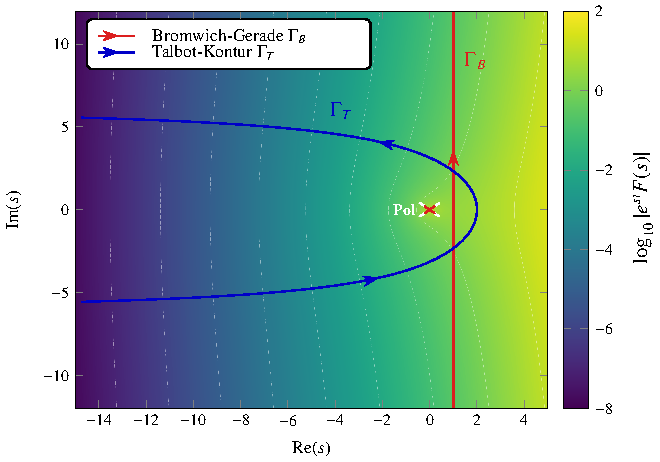
\includegraphics{papers/laplace/images/betrags_landschaft.pdf}
    \caption{Betragslandschaft $|e^{st}F(s)|$ über der komplexen
    $s$-Ebene für $F(s) = \frac{1}{s}$ zur Zeit $t = 1$ in
    logarithmischer Farbskala.
    Die Bromwich-Gerade (rot) verläuft auf konstanter Höhe durch das
    oszillierende Gebiet, während die Talbot-Kontur (blau) die
    Singularität umschliesst und beidseitig ins exponentiell tiefe Tal
    der linken Halbebene abtaucht.}
    \label{laplace:fig:betrags_landschaft}
\end{figure}
